\documentclass[11pt]{myclass}
\usepackage[margin=1in]{geometry}
\usepackage{mathptmx}
\usepackage{color}
\usepackage{hyperref}
\usepackage{verbatim}
\usepackage{amssymb}
\usepackage{algorithm, algorithmic}


\newcommand{\breg}{\ensuremath{D_\phi}}
\newcommand{\sbreg}{\ensuremath{D_{s\phi}}}
\newcommand{\eps}{\varepsilon}

\title{Streaming algorithms for MEB under the Bregman divergences}
\author{Alexander Clemmer, Amirali Abdullah , John Moeller}
%\date{} % Activate to display a given date or no date (if empty),
         % otherwise the current date is printed 

\begin{document}
\maketitle

\section{Introduction}
Given a point set $P$, and a distance function $D$, the Minimum-Enclosing-Ball (MEB) problem is defined as follows: Find $\min_{c,r} D(p,c)$ s.t. $p\leq r$ for every $p \in P$. The basic purpose of an MEB is to calculate \emph{extent} of a data set. Additionally, the center of the MEB so located, 
is the point s.t maximal distortion over all elements of $P$ is minimized. We consider the MEB ball under the \emph{Bregman divergence}  $\breg$, that is:

\begin{equation}
 \breg(x,y) = \phi(x) - \phi(y) - \langle \nabla \phi(y), x-y\rangle
\end{equation}

We define our MEB balls to be left balls, i.e, the center is always the second argument of $\breg$. This has the benefit that left-balls are always convex, as the Bregman divergence is convex in it's first argument, and that certain intermediate minimization problems become simpler, as we shall see later.

Although our analysis in this report extends to any Bregman divergence, we run our experiments on the $KL$-divergence, defined as :

\begin{equation}
D_{\text{kl}}(a,b) = \sum_{i=1}^{d} a_i \log \frac{a_i}{b_i} - (a_i - b_i)
\end{equation}

We use the $KL$-divergence because it is perhaps the most important Bregman divergence in practice, is easy to compute analytically, is convex in both arguments, and also has the most common challenging properties in analyzing Bregman diverences, i.e, distances and curvature going to infinity sharply (near the axes). 

\section{Related work}
 For $P$ in general position, and $D$ is the Euclidean distance $l_2$, there always exist some $d+1$ points that support the MEB of $P$. This is then a discrete problem, and can naively be solved in $O(n^{d+1})$ time. An exact solution can also be found in expected linear time, as first demonstrated by Welzl \cite{exact}. The problem can also be cast as one of approximation, and it is known that there exist core-sets for the Euclidean case as shown by Badoiu and Clarkson \cite{bc}.

The streaming setting denotes that we are constrained to space independent of $n$, and that we can only read our points sequentially (for the sake of this report, we only consider single-pass algorithms). The problem cannot be solved exactly in this setting, and so we try to find approximation algorithms, i.e, given some error parameter $\eps$ , find a ball $B(c,r)$ s.t $D(p,c) \leq r, \forall p$ and $r \leq (1+\eps)r_{\text{opt}}$.
Chan and Zarrabi-Zadeh give a simple streaming algorithm that obtains a $1.5$ approximate answer with $O(d)$ space (\cite{onepointfive}).
 Agarwal and  Sharathkumar present a somewhat more involved algorithm with $\eps > 0.22$ approximation that uses $O(d \frac{1}{\eps^3}\log \frac{1}{\eps} )$ storage (\cite{agarwal}). In our heuristic analysis, we will essentially be considering the analog of Chan's streaming algorithm, and its
generalization for Bregman divergences.

We note that the smallest enclosing ball probelm has been considered for Bregman divergences, albeit not in a streaming setting and without 
theoretically guaranteed convergence time. Nock and Nielsen present algorithms for generalizing both the Welzl algorithm \cite{bwz} as well as that of Badoui Clarkson \cite{bbc}, and in fact we implement the latter result to give us our baseline estimate of the optimal radius MEB.  

\section{Main algorithms}
We implemented three algorithms. One is the non-streaming base-line estimate of exact MEB derived from the paper of Nock and Nielsen \cite{bbc}. This was important to do so as to allow us to comapre the performance of our streaming analysis.

\begin{algorithm}
  \caption{Nielsen \& Nock Algorithm for divergences convex in both arguments}
  \begin{algorithmic}
    \STATE $n$ points, $p_1 \ldots p_n$, $t = T$
    \STATE Read point $c = p_i$ at random. 
    \REPEAT 
      \STATE Let $s$ be farthest point from $c$
      \STATE $c \leftarrow \frac{t}{t+1} c + \frac{1}{t+1} s$
    \UNTIL $t = 0$
    \STATE $r = d(p_i, c)$ for $p_i$ farthest from $c$
    \STATE Return $c, r$
  \end{algorithmic}
  \label{bbalgo}
\end{algorithm}

The second one is the most trivial algorithm, which simply takes first point as center and extends it at each step.

\begin{algorithm}
  \caption{Find MEB trivial}
  \begin{algorithmic}
    \STATE Read a stream of $n$ points, $p_1 \ldots p_n$. 
    \STATE Let $c = p_1$, $r = 0$, $i =2$
    \REPEAT 
    \STATE Read point $p_i$ from stream. 
    \IF{$\breg(p_i,c) >r$ }
      \STATE Let $r = \breg(p_i,c)$
    \ENDIF 
    \STATE $i = i+1$
    \UNTIL $i > n$
    \STATE Return $c,r$
  \end{algorithmic}
  \label{trivial}
\end{algorithm}

Note that algorithm \ref{trivial} guarantees us a $2$ approx for the Euclidean case by the triangle inequality which is often a reasonable ball-park estimate for many applications. However, one would expect this to be poor for Bregman divergences where the triangle inequality may be violated to an arbitrarily bad degree, and in our results we shall demonstrate that this is indeed the case.

The third one is the generalization of the algorithm given by Chan and Zarrabi-Zadeh \cite{onepointfive}. We note that this is not immediate, and is the main theoretical contribution of our report.

\begin{algorithm}
  \caption{Find MEB Ext-ball}
  \begin{algorithmic}
    \STATE Read a stream of $n$ points, $p_1 \ldots p_n$. 
    \STATE Let $c = p_1$, $r = 0$, $i =2$
    \REPEAT 
    \STATE Read point $p_i$ from stream. 
    \IF{$\breg(p_i,c) >r$ }
      \STATE Find $c_{\text{new}}$, $r_{\text{new}}$ s.t $B(c,r) \subset B(c_{\text{new}}, r)$
	  \STATE $c = c_{\text{new}}, r = r_{\text{new}}$ 
	\ENDIF
    \STATE $i = i+1$
    \UNTIL $i > n$
    \STATE Return $c,r$
  \end{algorithmic}
  \label{extendalgo}
\end{algorithm}

Note that the key step here is given a $B(c,r)$ and a new point $p_i$ that lies outside of it, we need to find an extension of the ball that contains both the point $p$ AND the original ball. In our next section, we descibe how to do this.

\section{Extending ball}
We first note given a left-ball $B(c,r)$ and point $p$, how to find  $\max_{x \in B(c,r)} \breg(x,p)$. 
Note that since the Bregman divergence is convex in the first argument, this is a convex optimization problem. We can set up the Lagrange multipliers as done by Cayton (see \cite{cayton} for details) and a simple computation shows that the solution of the nearest and farthest point
in $B(c,r)$ to $p$ is satisfied by $x$ s.t. $\breg(x,c) = r$, $\nabla \phi(x) = \theta \nabla \phi(c) + (1 - \theta) \nabla \phi(p)$. That is,
the farthest point ($p_{\text{far}}$) and the nearest point $(p_{\text{near}})$ both lie along the straight line joining $c$ and $p$ in the
gradient space.

\begin{figure}[H]
  \begin{center}
    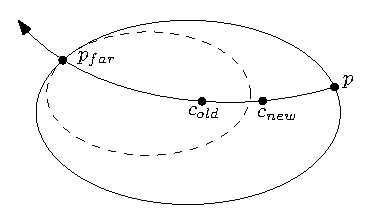
\includegraphics[scale=1.2]{../figures/interpolate}
  \end{center}
  \caption{Finding $c_{\text{new}}$}
  \label{Trivial fails}
\end{figure}

This immediately suggests a straightforward algorithm for computing $c_{\text{new}}$ - simply do a binary search along the straight line joining $\nabla \phi(c)$ and $\nabla \phi(p)$, and find $c_{\text{new}}$ s.t $\breg(p_{\text{far}}, c_{\text{new}}) = \breg(p, c_{\text{new}})$. Although we do not have a proof that our extend ball approach is indeed the minimal radius new ball that encloses both $B(c,r)$ and $p$, our experimental results support the conjecture strongly.
 
\section{Experimental Results}
We run our data over $3$ types of point sets. The first group of data sets is a points spread exponentially far apart, and at growing rate. We observe that Algorithm \ref{trivial} performs poorly as expected and indeed tends to arbitrarily bad approximation ratios as we increase the exponential gap of our points. However, our Algorithm \ref{extendalgo} performs fine and matches the exact algorithm \ref{bbalgo}. We plot the following graph where each point represents the approximation quality of a data set, and increasing x-coordinate indicates greater exponential spread of a data set.

\begin{figure}[H]
  \begin{center}
    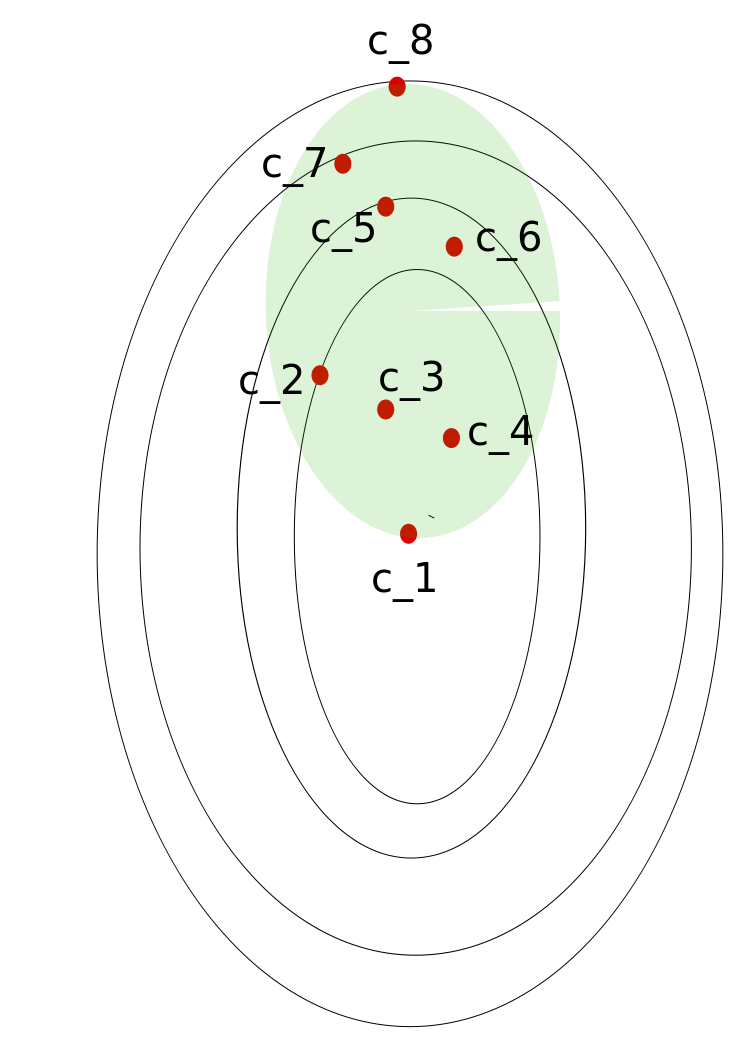
\includegraphics[scale = 0.2]{../figures/trivial_fail}
  \end{center}
  \caption{The green ball is the optimal ball and the contours are balls produced by Algorithm \ref{trivial}}
\end{figure}

\begin{figure}[H]
  \begin{center}
    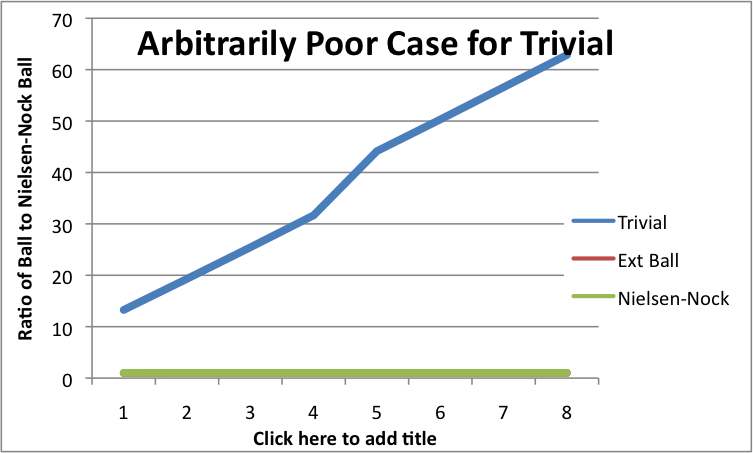
\includegraphics[scale = 0.8]{../figures/trivial_poor.png}
  \end{center}
  \caption{Note the poor performance of the trivial algorithm}
\end{figure}

For our second type of data set, we pick points regularly spread over the unit hyper cube (in the first orthant) . Due to numerical issues and overflows, we made sure the points were bounded away from the axes which is where the $kl$-divergence tends to infinity. We found that for these types of data sets , increasing $d$ has little to no impact on the quality of approximation obtained. This is not surprising, in the light of \cite{onepointfive}, in which the worst case approximation bounds do not involve $d$.

\begin{figure}[H]
  \begin{center}
    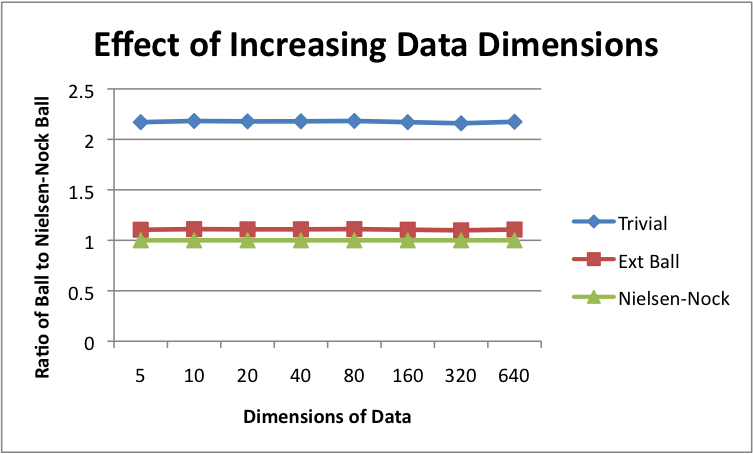
\includegraphics[scale = 0.8]{../figures/inc_dimensions.png}
  \end{center}
  \caption{Note the essentially flat performance with increasing dimensionality }
  \label{incdim}
\end{figure}

Finally, we considered our third type of data set, points spread uniformly around the boundary of a ball. This is the point set that realizes the $1.5$ lower bound for the Euclidean case (\cite{onepointfive}), and indeed realizes our worst results for Algorithm \ref{extendalgo} of $1.6$. We obtained this for points spread around the boundary of a Bregman ball, both over a small domain (where a ball is more roughly spherical) and also near the an axis ( where a ball is much more anisotropic and elliptical. In both cases, surprisingly, our Algorithm \ref{extendalgo} attained a $1.6$ bound. It remains open whether taking more anomalous balls 
or regions will exhibit an arbitrarily bad bound for Algorithm \ref{extendalgo} on the lines of Algorithm \ref{trivial} or whether
there is indeed a worst case performance bound.

\begin{figure}[H]
  \begin{center}
    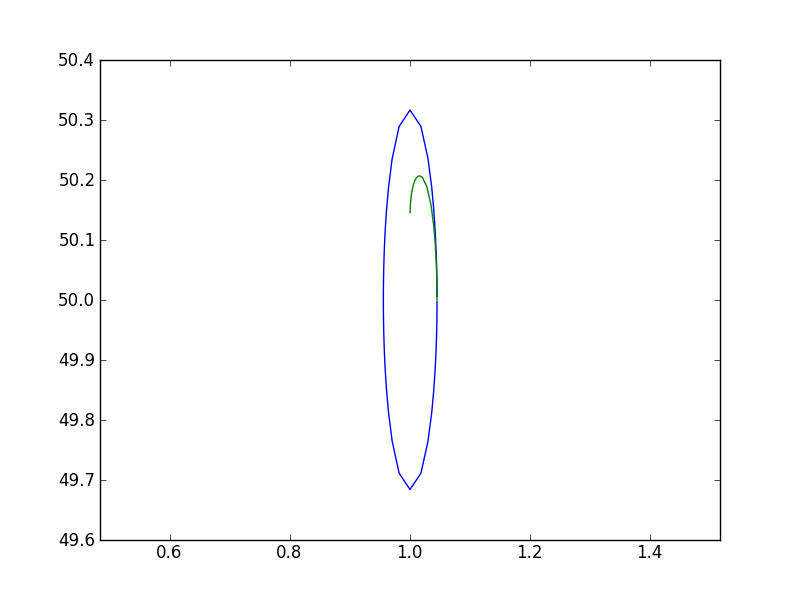
\includegraphics[scale = 0.6]{../figures/ellipse-bad.png}
  \end{center}
  \caption{Data arranged around a ball. The approximate center converges to a point far from the real center}
\end{figure}

\begin{figure}[H]
  \begin{center}
    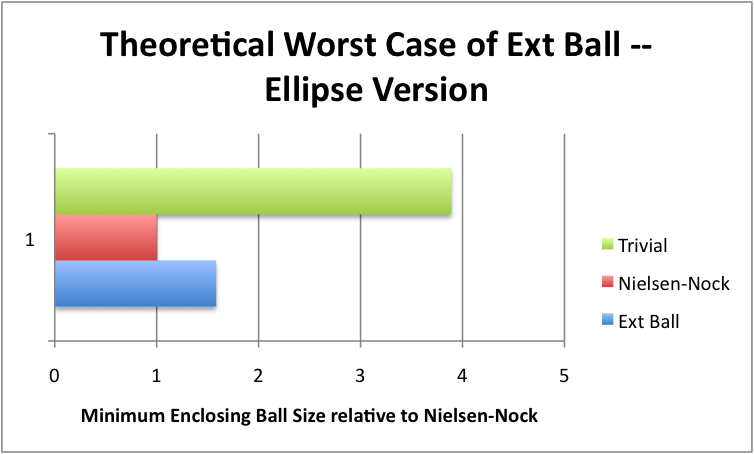
\includegraphics[scale = 0.8]{../figures/eb_worst.png}
  \end{center}
  \caption{A not too irregular Bregman ball}
  \label{ball}
\end{figure}
\begin{figure}[H]
  \begin{center}
    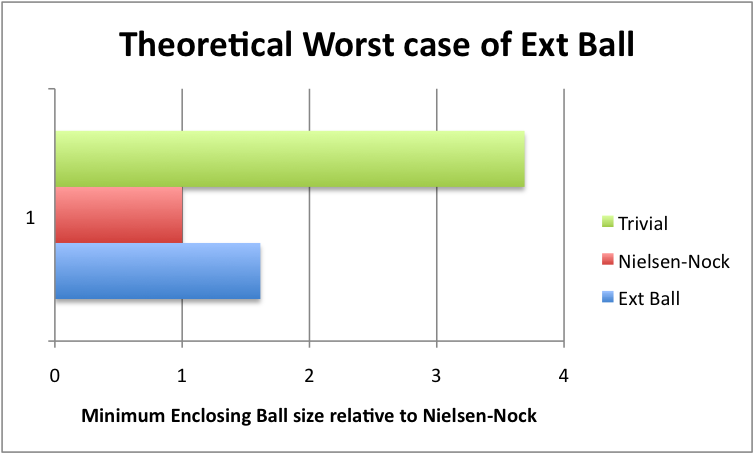
\includegraphics[scale = 0.8]{../figures/eb_worst_ellipse.png}
  \end{center}
  \caption{A highly anisotropic Bregman ball}
  \label{ellipse}
\end{figure}

\section{Further work}
Agarwal and Sharathkumar obtain better approximation guarantees than the ball extension of Chan and Zarrabi-Zadeh (\cite{onepointfive}) by essentially maintaining multiple coresets of the data. Before any further such extension, one key question is whether coresets even exist for the MEB under Bregman divergences. The conjecture in the theoretical community is that there is not, without a boundedness assumption, but there is no published result verifying the same.

Secondly, can we give theoretical upper bounds on the approximation quality of our heuristic in a bounded domain, using the fact that a Bregman diveregnce satisfies approximate triangle inequality over any bounded domain?

Thirdly, can we show a higher lower bound on approximation quality than the $1.22$ that holds for the Euclidean case if we allow unbounded domain?

\newpage
\bibliography{meb}
\bibliographystyle{acm}



\appendix

\section{Distribution of work}
John implemented the base-line algorithm \ref{bbalgo} for computing exact MEB (\cite{bbc}) as well as offer several helpful ideas
and suggestions for the theory component of this report.  

Alexander implemented our own algorithm \ref{extendalgo}, and ran the major experiments on our data sets as well as handling 
multiple tricky numerical and computational issues that arise at boundary cases.

Amir handled the major part of theoretical content and background, including the idea on how to extend the ball and construction of the
datasets.
\end{document}